\section{Methodology}

% TODO description

\subsection{Peripherals}

The external hardware required for developing the project will be described in detail.

\subsubsection{Tobii Pro Nano Eye Tracker}

\begin{figure}[ht]
    \centering
    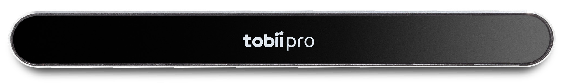
\includegraphics[width=0.4\textwidth]{images/tobii-pro-nano.png}
    \caption{Tobii Pro Nano Eye Tracker. Source: \citep{manual:tobiipronano}}
    \label{fig:tobii-eye-tracker}
\end{figure}

The Tobii Pro Nano Eye Tracker, shown above in figure \ref{fig:tobii-eye-tracker}, uses a corneal reflection, dark and bright pupil combination, one-camera system. It supports screen sizes up to 19 inches, introduces a 17 ms system latency. \citep{manual:tobiipronano}

It is characterized by its lightweight and compact form; which makes it easy to carry, and ultimately enabled an easier usability testing process. On the other hand, Tobii Eye Trackers are compatible with the \verb|tobii-research| SDK for python, which allows for controlling the device without the need for a graphical user interface.

This device prompted the idea for the project.

\subsubsection{Microphone}

The microphone serves as a mediator of interaction, enabling the capture of verbal cues essential for the analysis of words that then get turned into commands thanks to the natural language processing. It also serves as an way of qualitative data acquisition, for recording each participant response for usability testing.

\subsection{System Design}

The software developed 

\subsubsection{Software Architecture}

\begin{figure}[ht]
    \centering
    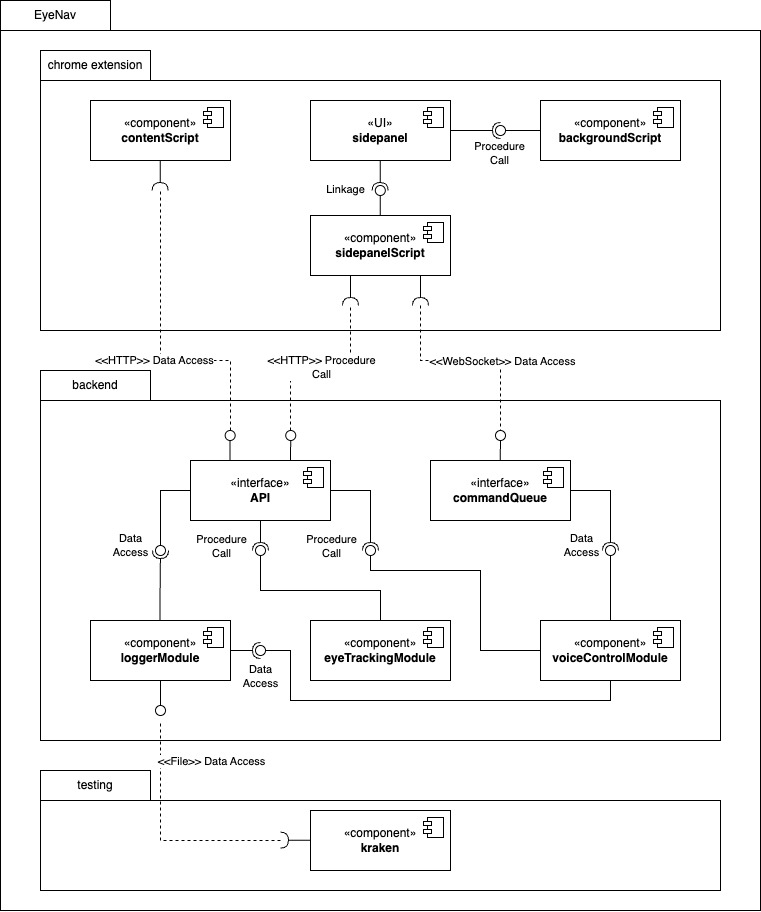
\includegraphics[width=0.85\textwidth]{images/components-diagram.jpg}
    \caption{Architecture described in components}
    \label{fig:components-diagram}
\end{figure}

\begin{figure}[ht]
    \centering
    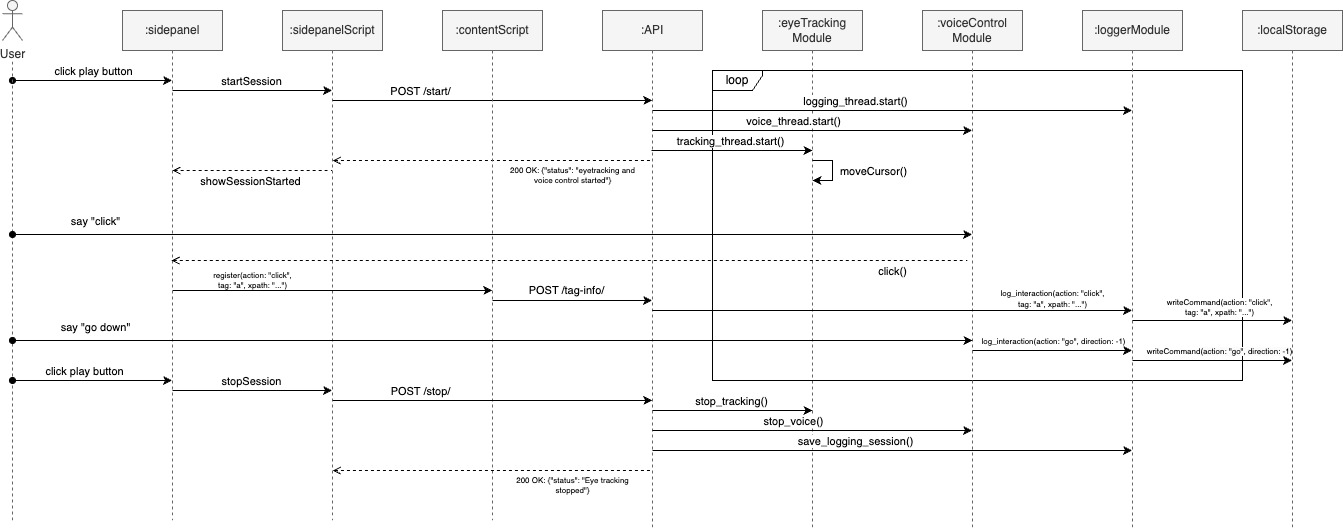
\includegraphics[width=0.85\textwidth]{images/sequence-diagram.jpg}
    \caption{An user clicking and scrolling sequence}
    \label{fig:sequence-diagram}
\end{figure}


\subsubsection{Chrome Extension}

\subsubsection{HTTP Server}

% -vosk voice recognition
% -tobii pro sdk

\subsubsection{Websockets}

\subsubsection{Testing}





